\section{Experiments and Results}
\label{sec:experiments}

% We report results on multiple splits of the data.
First, we report the overall consistency performances, per graph, as describe in Section \ref{sec:eval}.
The results for the different models are summarized in Table \ref{tab:entailment-main}.
% That is, the overall successful prediction of the entailed pattern, divided by the overall connection. This measurement can also be seen as a weighted average, since every edge gets a score averaged by the number of base patterns that were predicted correctly.
That is, the p1, 



\begin{table*}[t]
% \small
    \centering
\resizebox{1\textwidth}{!}{%
\begin{tabular}{lrrrrrrrr}
\toprule
                              Pattern &  bert-base &  bert-large &  bert-large-wwm &  roberta-base &  roberta-large &  albert-base &  albert-xxlarge &   n \\
\midrule
                          instance of &       0.40 &        0.47 &            0.44 &          0.30 &           0.38 &         0.35 &            0.36 &  21 \\
                             employer &       0.55 &        0.38 &            0.31 &          0.34 &           0.53 &         0.40 &            0.29 &   4 \\
               country of citizenship &       0.70 &        0.71 &            0.68 &          0.73 &           0.71 &         0.54 &            0.62 &  16 \\
                         record label &       0.32 &        0.26 &            0.29 &          0.33 &           0.35 &         0.35 &            0.48 &  37 \\
                                genre &       0.49 &        0.49 &            0.39 &          0.40 &           0.33 &         0.22 &            0.27 &  11 \\
                        position held &       0.60 &        0.48 &            0.46 &          0.40 &           0.33 &         0.50 &            0.34 &   6 \\
                    country of origin &       0.61 &        0.62 &            0.58 &          0.59 &           0.57 &         0.43 &            0.42 &  29 \\
                          subclass of &       0.75 &        0.76 &            0.79 &          0.70 &           0.73 &         0.69 &            0.75 &   4 \\
              applies to jurisdiction &       0.89 &        0.90 &            0.92 &          0.84 &           0.87 &         0.91 &            0.87 &   4 \\
                   shares border with &       0.54 &        0.54 &            0.56 &          0.38 &           0.47 &         0.45 &            0.55 &   9 \\
                              country &       0.83 &        0.84 &            0.83 &          0.77 &           0.77 &         0.74 &            0.73 &   3 \\
                    official language &       0.77 &        0.84 &            0.84 &          0.67 &           0.78 &         0.44 &            0.66 &  12 \\
                              capital &       0.72 &        0.78 &            0.81 &          0.50 &           0.67 &         0.59 &            0.76 &  14 \\
             language of work or name &       0.66 &        0.69 &            0.65 &          0.59 &           0.64 &         0.48 &            0.40 &  15 \\
                     original network &       0.25 &        0.28 &            0.29 &          0.27 &           0.30 &         0.26 &            0.25 &  28 \\
 position played on team / speciality &       0.29 &        0.31 &            0.32 &          0.32 &           0.36 &         0.49 &            0.56 &   9 \\
                headquarters location &       0.55 &        0.51 &            0.63 &          0.47 &           0.58 &         0.42 &            0.47 &  10 \\
                           instrument &       0.35 &        0.50 &            0.55 &          0.38 &           0.48 &         0.68 &            0.40 &  11 \\
                         manufacturer &       0.82 &        0.86 &            0.87 &          0.58 &           0.70 &         0.75 &            0.83 &  25 \\
          twinned administrative body &       0.67 &        0.69 &            0.66 &          0.50 &           0.54 &         0.50 &            0.57 &   8 \\
                            continent &       0.87 &        0.91 &            0.86 &          0.60 &           0.75 &         0.90 &            0.86 &   4 \\
                            developer &       0.61 &        0.60 &            0.77 &          0.64 &           0.73 &         0.55 &            0.69 &  16 \\
                              part of &       0.54 &        0.57 &            0.60 &          0.51 &           0.48 &         0.64 &            0.58 &   2 \\
                             owned by &       0.32 &        0.44 &            0.43 &          0.32 &           0.36 &         0.28 &            0.34 &   4 \\
                location of formation &       0.47 &        0.52 &            0.55 &          0.50 &           0.49 &         0.35 &            0.32 &  17 \\
                        field of work &       0.20 &        0.23 &            0.20 &          0.19 &           0.22 &         0.48 &            0.26 &  26 \\
                           capital of &       0.87 &        0.92 &            0.94 &          0.77 &           0.89 &         0.85 &            0.91 &  14 \\
                           occupation &       0.22 &        0.35 &            0.27 &          0.22 &           0.27 &         0.17 &            0.14 &  16 \\
                             location &       0.48 &        0.49 &            0.57 &          0.42 &           0.46 &         0.46 &            0.50 &  27 \\
                       place of death &       0.29 &        0.38 &            0.25 &          0.33 &           0.23 &         0.16 &            0.20 &   8 \\
                             religion &       0.29 &        0.34 &            0.46 &          0.34 &           0.32 &         0.19 &            0.36 &   3 \\
                       place of birth &       0.37 &        0.41 &            0.40 &          0.32 &           0.36 &         0.31 &            0.35 &  14 \\
                            member of &       0.79 &        0.85 &            0.82 &          0.80 &           0.87 &         0.83 &            0.81 &  15 \\
                        work location &       0.80 &        0.72 &            0.63 &          0.57 &           0.63 &         0.41 &            0.41 &   9 \\
                          named after &       0.76 &        0.71 &            0.75 &          0.54 &           0.64 &         0.66 &            0.73 &  20 \\
 original language of film or TV show &       0.86 &        0.90 &            0.80 &          0.64 &           0.67 &         0.63 &            0.52 &   6 \\
 \midrule
 Average & 0.57 & 0.59 & 0.59 & 0.49 & 0.54 & 0.50 & 0.52 & 13.25 \\
 
\bottomrule
\end{tabular}
}
    \caption{Consistency results for the different relations. Reporting the average accuracy on different LMs, along with the number of patterns per relation.}
    \label{tab:entailment-main}
\end{table*}

\begin{table*}[t]
% \small
    \centering
\resizebox{1\textwidth}{!}{%
\begin{tabular}{lrrrrrrr}
\toprule
{} &  bert-base &  bert-large &  bert-large-wwm &  roberta-base &  roberta-large &  albert-base &  albert-xxlarge \\
\midrule
syn   &             0.50 &              0.53 &                                 0.53 &          0.44 &           0.48 &            0.44 &               0.45 \\
lex   &             0.56 &              0.59 &                                 0.58 &          0.51 &           0.54 &            0.52 &               0.49 \\
both  &             0.72 &              0.72 &                                 0.72 &          0.67 &           0.68 &            0.70 &               0.63 \\ \midrule
total &             0.52 &              0.54 &                                 0.54 &          0.45 &           0.50 &            0.46 &               0.46 \\
\bottomrule
\end{tabular}


}
    \caption{Consistent results aggregated on the different relations, by the different splits.}
    \label{tab:entailment-splits}
\end{table*}

\begin{table*}[t]
% \small
    \centering
\resizebox{1\textwidth}{!}{%
\begin{tabular}{llrrrrrrr}
\toprule
     type & index &  bert-base-cased &  bert-large-cased &  bert-large-cased-wwm &  roberta-base &  roberta-large &  albert-base &  albert-xxlarge \\
\midrule
\multirow{3}{*}{consistency} & 1-1 &             0.76 &              0.82 &                                 0.84 &          0.58 &           0.73 &            0.66 &               0.80 \\
     & N-1 &             0.55 &              0.56 &                                 0.57 &          0.48 &           0.51 &            0.46 &               0.48 \\
     & N-M &             0.43 &              0.47 &                                 0.46 &          0.39 &           0.44 &            0.44 &               0.40 \\
\cline{1-9}
\multirow{3}{*}{syntactic} & 1-1 &             0.75 &              0.81 &                                 0.83 &          0.57 &           0.72 &            0.66 &               0.79 \\
     & N-1 &             0.53 &              0.55 &                                 0.56 &          0.46 &           0.49 &            0.44 &               0.47 \\
     & N-M &             0.41 &              0.45 &                                 0.44 &          0.38 &           0.43 &            0.42 &               0.40 \\
\cline{1-9}
\multirow{3}{*}{lexical} & 1-1 &             0.85 &              0.88 &                                 0.89 &          0.67 &           0.80 &            0.75 &               0.86 \\
     & N-1 &             0.59 &              0.60 &                                 0.62 &          0.55 &           0.57 &            0.51 &               0.51 \\
     & N-M &             0.45 &              0.53 &                                 0.48 &          0.40 &           0.44 &            0.52 &               0.39 \\
\cline{1-9}
\multirow{3}{*}{both} & 1-1 &             0.59 &              0.76 &                                 0.83 &          0.16 &           0.49 &            0.46 &               0.73 \\
     & N-1 &             0.75 &              0.76 &                                 0.74 &          0.69 &           0.72 &            0.72 &               0.69 \\
     & N-M &             0.68 &              0.66 &                                 0.68 &          0.64 &           0.64 &            0.68 &               0.54 \\
\bottomrule
\end{tabular}

}
    \caption{Consistent results aggregated on the different relations, by the different splits.}
    \label{tab:entailment-splits}
\end{table*}

\begin{figure*}[t!]
\centering

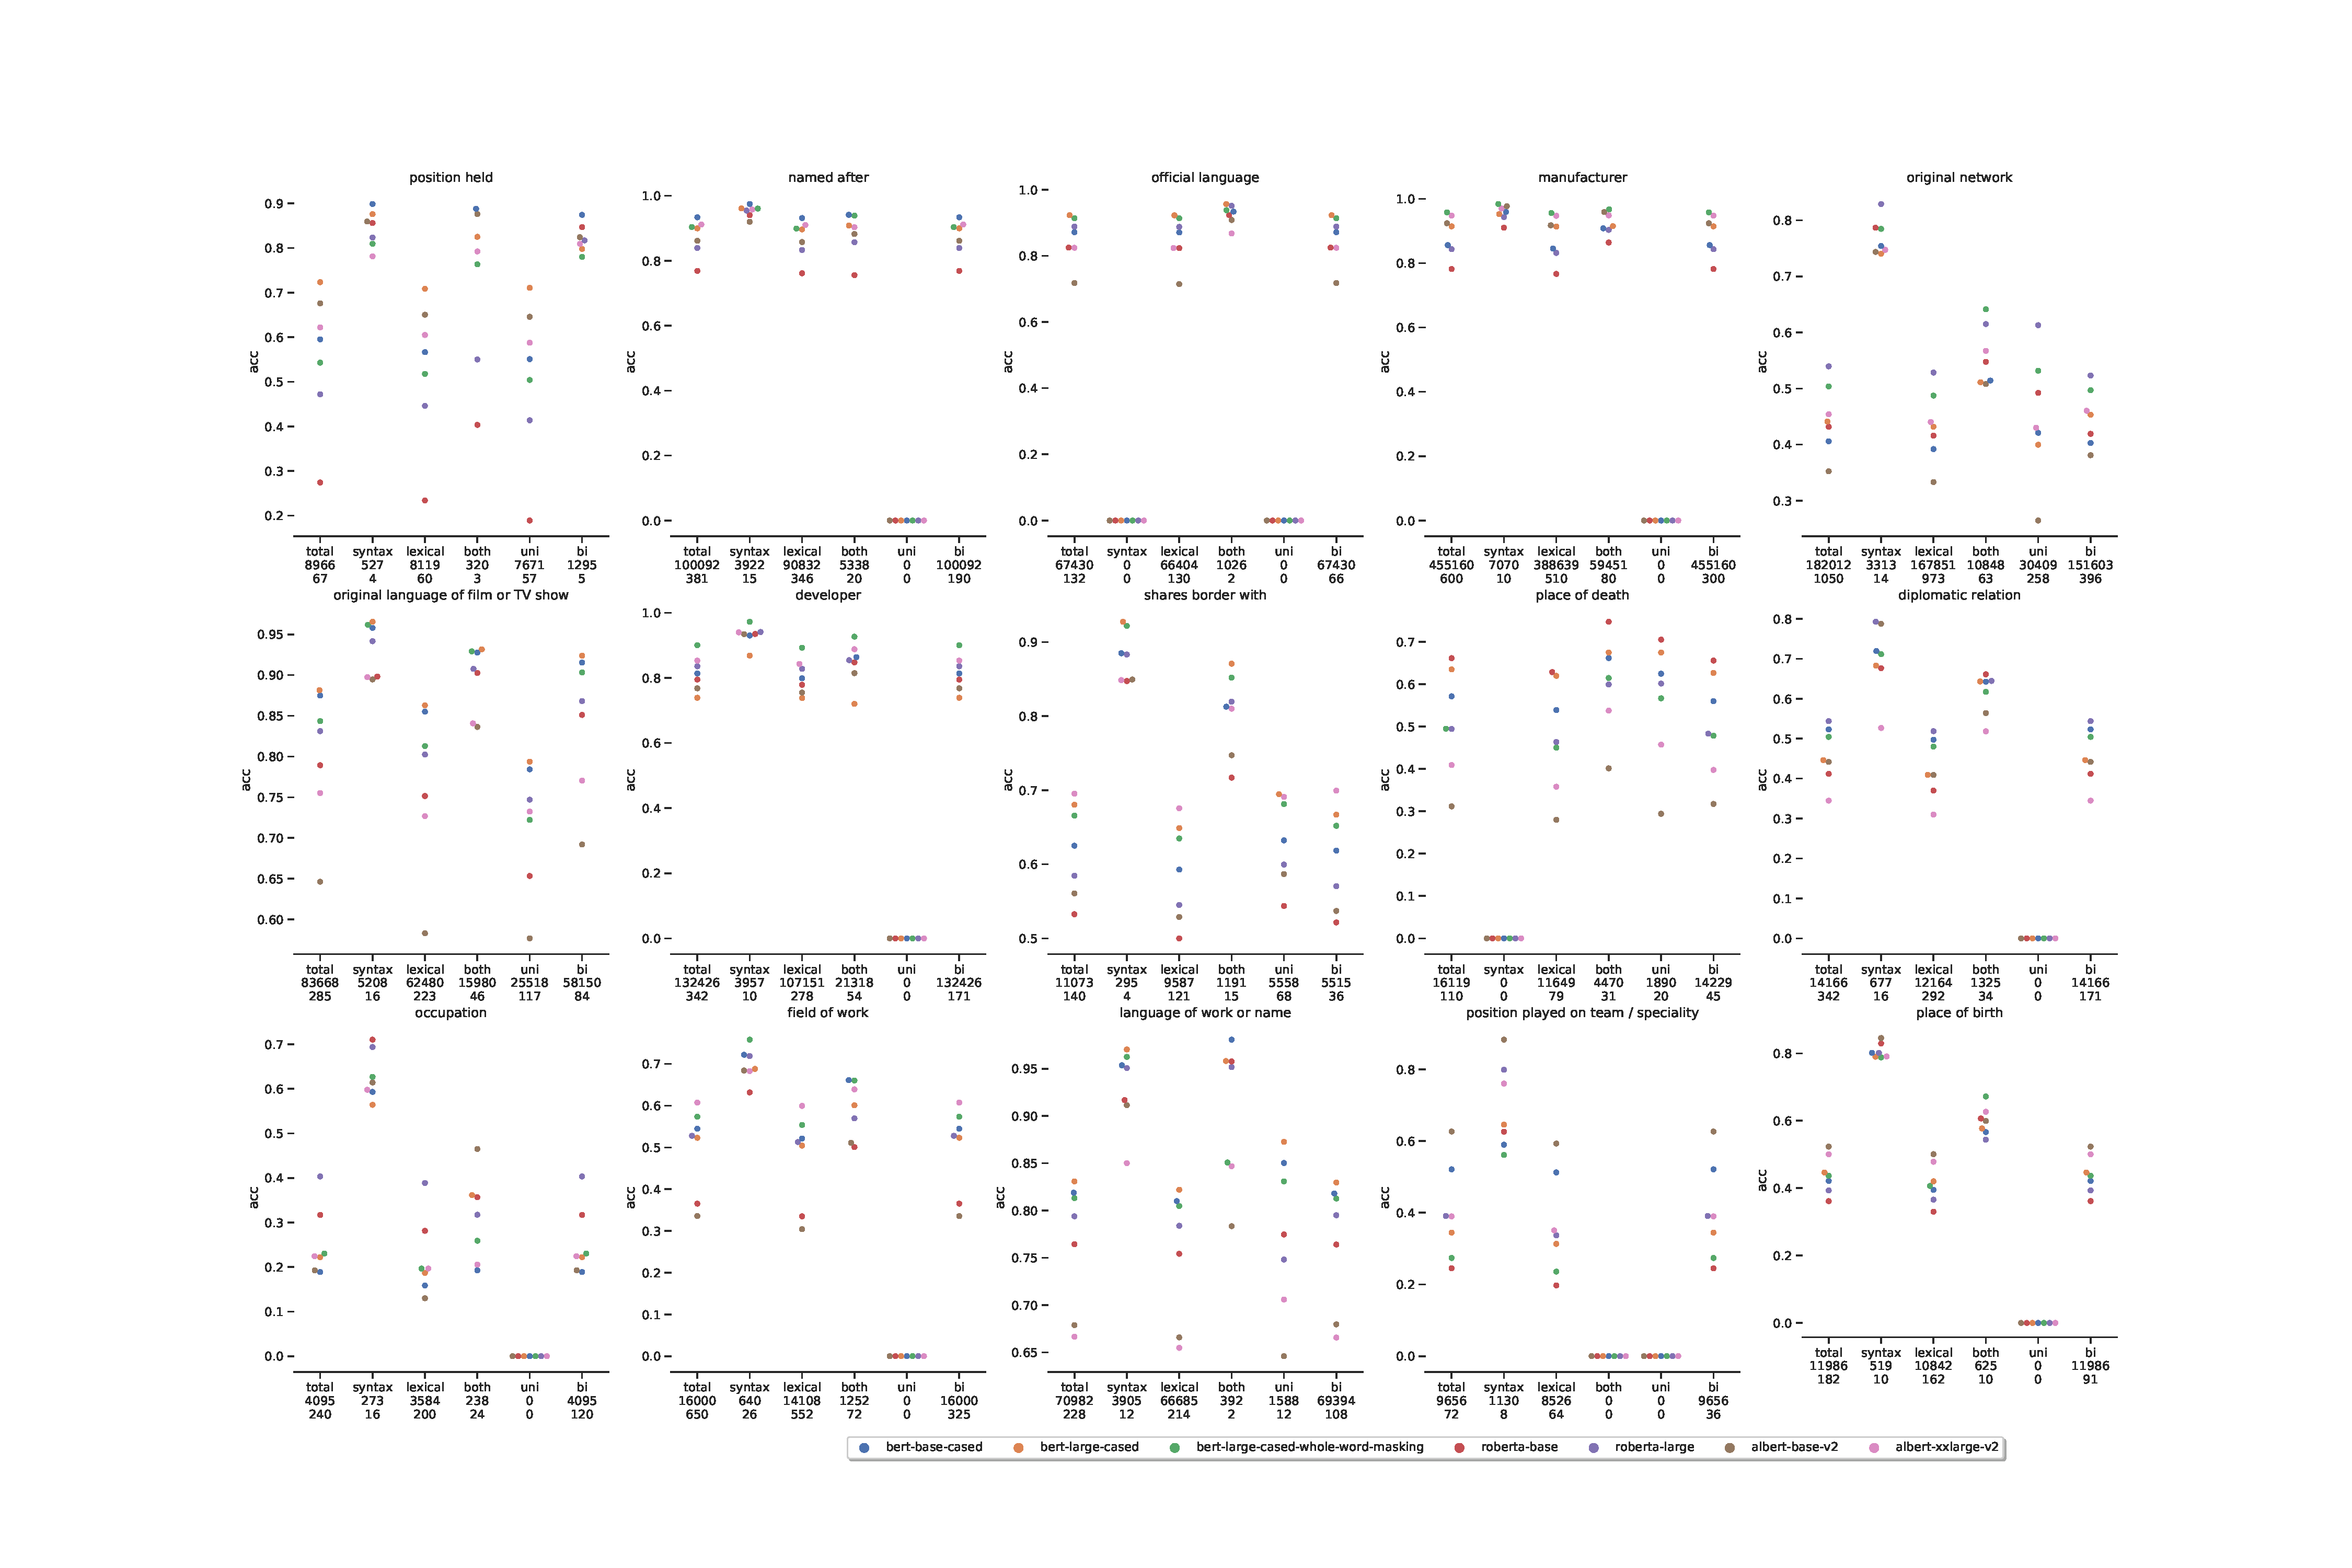
\includegraphics[width=1.\textwidth]{figures/results}

\caption{Results summary, by relation, by split.}
\label{fig:resuls}
% \vspace{-6mm}
\end{figure*}